\documentclass{TIJMUjiaoanLL}
\pagestyle{empty}


\begin{document}


%课程名称
\kecheng{Linux系统概论}
%课程内容
\neirong{软件安装\ /\ 第19章}
%教师姓名
\jiaoshi{伊现富}
%职称
\zhicheng{讲师}
%教学日期(格式:XXXX年XX月XX日XX时-XX时)
\riqi{2019年6月4日13:30-15:10}
%授课对象(格式:XXX系XXXX年级XX班(硕/本/专科))
\duixiang{生物医学工程与技术学院2017级生信班(本)}
%听课人数
\renshu{28}
%授课方式
\fangshi{理论讲授}
%学时数
\xueshi{2}
%教材版本
\jiaocai{Unix入门经典,第1版}


%教案首页
\firstHeader
\maketitle
\thispagestyle{empty}

\mudi{
\begin{itemize}
  \item 掌握APT的使用方法,Yum的使用方法,GPL的思想,源代码安装软件的主要步骤。
  \item 熟悉dpkg的使用方法,RPM的使用方法,命令行下载软件的方法,脚本安装软件的方法。
  \item 了解各种开源许可证,源代码编译的过程。
  \item 自学其他的二进制软件包管理方法。
\end{itemize}
}

\fenpei{
\begin{itemize}
  \item (5')引言与导入:介绍软件包管理的概念、常见的软件包,总结Linux中的二进制软件包管理系统。
  \item (45')二进制软件包管理:详细讲解dpkg和APT、RPM和Yum进行软件包管理的命令,简要比较各种二进制软件包的管理。
  \item (40')源代码安装:介绍常见的开源许可证,讲解GPL的思想,介绍选择和下载软件的方法,讲解从源代码编译和安装软件的步骤。
  \item (5')脚本安装:介绍通过脚本安装软件的过程。
  \item (5')总结与答疑:总结授课内容中的知识点与技能,解答学生疑问。
\end{itemize}
}

\zhongdian{
\begin{itemize}
  \item 重点:APT和Yum的使用,从源代码安装软件的步骤。
  \item 难点:dpkg和RPM的使用。
  \item 解决策略:通过实例讲解与操作演示帮助学生理解、记忆。
\end{itemize}
}

\waiyu{
  \vspace*{-10pt}
  \begin{multicols}{2}
    开放源代码(open source)

    自由软件(free software)
  \end{multicols}
  \vspace*{-10pt}
}

\fuzhu{
\begin{itemize}
  \item 多媒体:dpkg和APT、RPM和Yum二进制软件包的管理命令,各种二进制软件包管理的比较,开源许可证。
  \item 板书:从源代码安装软件的步骤。
  \item 演示:dpkg和APT、RPM和Yum的使用。
\end{itemize}
}

\sikao{
  \vspace*{-10pt}
  \begin{multicols}{2}
  \begin{itemize}
    \item Ubuntu和CentOS等常见Linux发行版使用的软件包管理系统是什么?
    \item 列举dpkg和APT软件包管理中的常用命令及其作用。
    \item 列举RPM和Yum软件包管理中的常用命令及其作用。
    \item 列举几个常见的开放源代码许可证。
    \item GPL授予程序使用者哪些“自由”?
    \item 通过源代码安装软件的基本步骤是什么?
  \end{itemize}
  \end{multicols}
  \vspace*{-10pt}
}

\cankao{
\begin{itemize}
  %\item (美)Paul Love,Joe Merlino\ 等著,张楚雄,许文昭\ 译。Unix入门经典,清华大学出版社,2006。
  \item (美)Harley Hahn\ 著,张杰良\ 译。Unix \& Linux大学教程,清华大学出版社,2010。
  \item 鸟哥\ 著,王世江\ 改编。鸟哥的Linux私房菜——基础学习篇(第三版),人民邮电出版社,2010。
  \item 维基百科等网络资源。
\end{itemize}
}

\firstTail


%教案续页
\newpage
\otherHeader

\begin{enumerate}
  \item
    引言与导入(5分钟)\textcolor{red}{(通过和Windows中软件、软件管理的比较进行导入)}
    \begin{enumerate}
      \item 软件包管理系统
	\begin{itemize}
\parpic[fr]{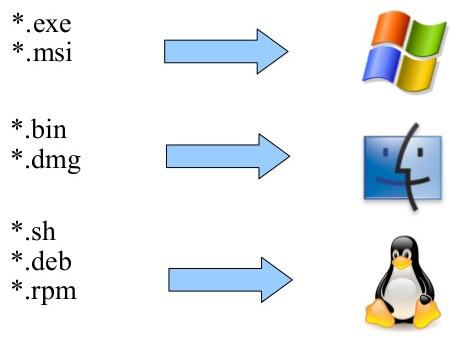
\includegraphics[width=8cm]{c6_software.png}}
	  \item 自动安装卸载、配置和升级软件包的工具组合
	  \item 大大简化在Linux发行版中安装软件的过程
	\end{itemize}
      \item 软件包
	\begin{itemize}
	  \item 二进制包(预编译的软件包)
	    \begin{itemize}
	      \item deb软件包
	      \item rpm软件包
	    \end{itemize}
	  \item 源代码安装包
	  \item 脚本安装包
	\end{itemize}
      \item 二进制包管理系统
	\begin{itemize}
          \item dpkg及其前端APT:Ubuntu, Debian, Deepin
          \item RPM及其前端Yum:Red Hat Enterprise Linux, CentOS, Fedora
          \item ZYpp及其前端Zypper:SUSE, openSUSE
          \item 其他:urpmi(Mandriva Linux, Mageia Linux, ROSA Linux),pacman(Arch Linux),slapt-get(Slackware),Portage(Gentoo)
	\end{itemize}
    \end{enumerate}

  \item 二进制软件包管理(45分钟)
    \begin{enumerate}
      \item dpkg与APT
	\begin{enumerate}
	  \item 简介
	    \begin{itemize}
	      \item dpkg:底层工具,Debian软件包管理器的基础
	      \item APT:dpkg的前端,Debian及其派生发行版的软件包管理器
	      \item Aptitude:APT的前端(文字终端)
	    \end{itemize}
	  \item \textcolor{red}{\textbf{【难点】}}dpkg\textcolor{red}{(实例讲解、操作演示)}
	    \vspace*{-10pt}
	    \begin{figure}[h]
	      \centering
	      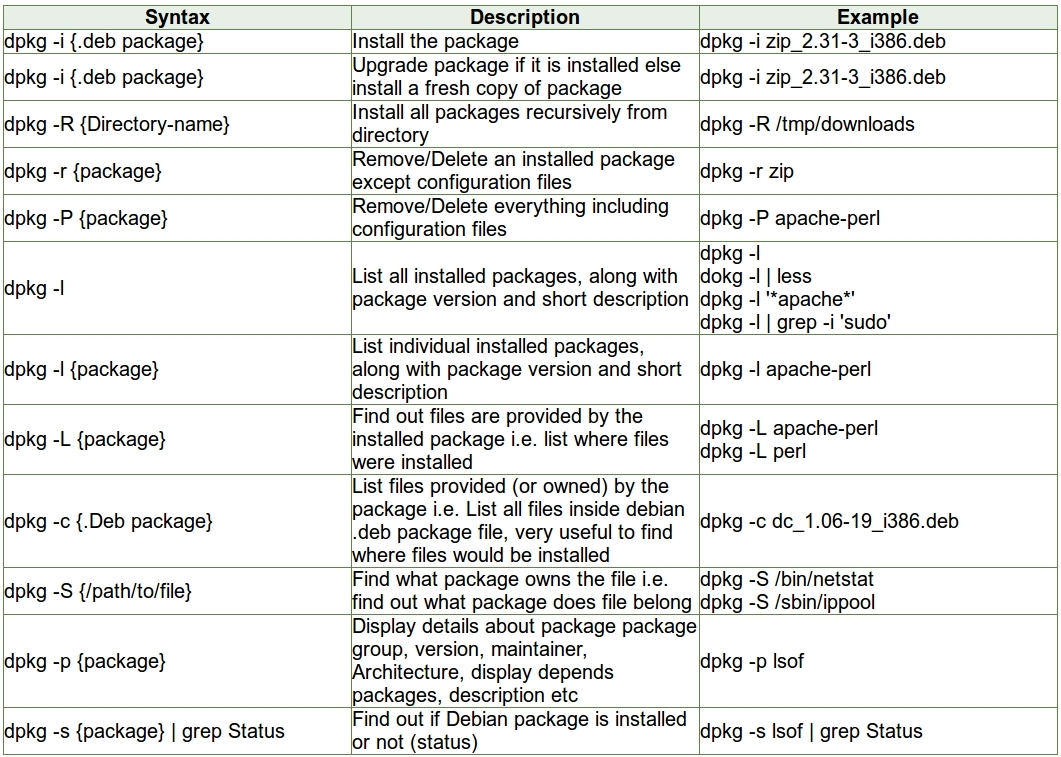
\includegraphics[width=14.5cm]{c6_dpkg_01.png}
	    \end{figure}
	    \vspace*{-10pt}

\otherTail
\newpage
\otherHeader

	  \item \textcolor{red}{\textbf{【重点】}}APT\textcolor{red}{(实例讲解、操作演示)}
	    \begin{itemize}
\parpic[fr]{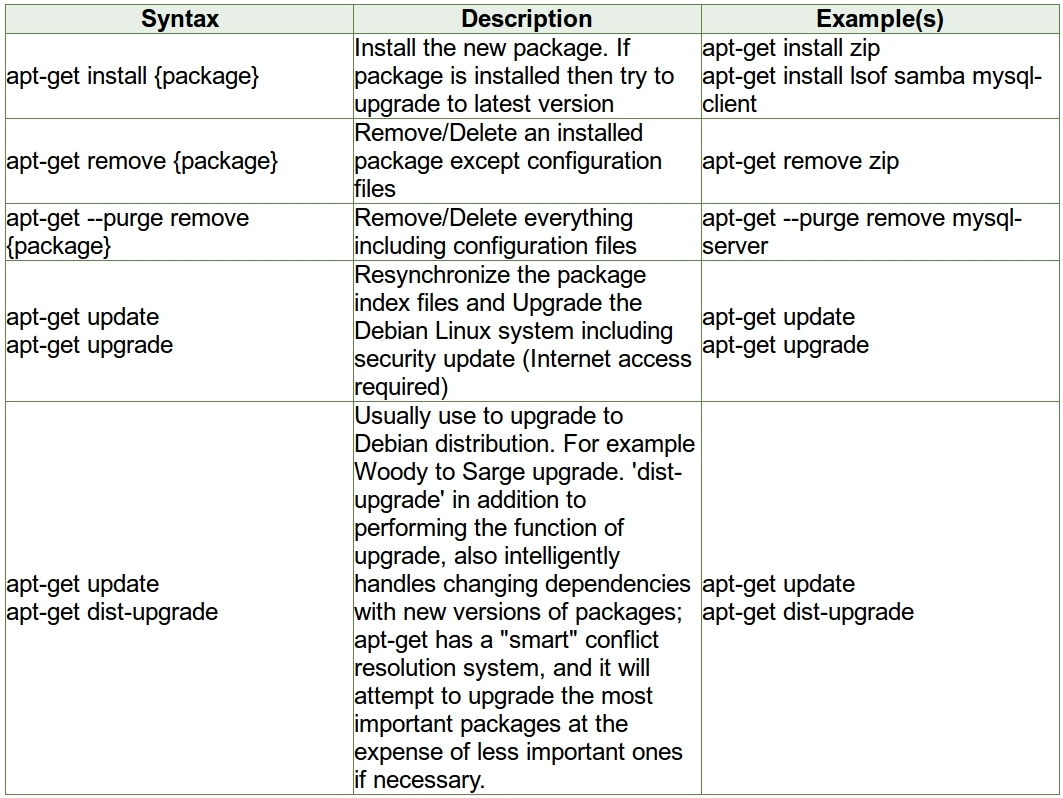
\includegraphics[width=8.3cm,height=7cm]{c6_apt_01.png}}
	      \item apt-get:负责软件包的在线安装与升级,底层对deb包的处理还是用的dpkg,解决依赖关系
              \item apt-cache:用来查询软件包的状态和依赖关系
              \item apt-file:负责查询软件包名称和软件包包含的文件(值得注意的是它要自己同步)
              \item apt-cross:负责为交叉编译的软件包的安装与编译等
	      \item apt-offline:可以离线安装软件包
              \item apt-build:可以简化源代码编译
            \end{itemize}
	  \item PPA
	    \begin{enumerate}
              \item 添加PPA源:sudo add-apt-repository ppa:user/ppa-name
	      \item 更新所有源:sudo apt-get update
	      \item 安装软件:sudo apt-get install <package\_name>
	    \end{enumerate}
	\end{enumerate}
      \item RPM与Yum
	\begin{enumerate}
	  \item 简介
	    \begin{itemize}
%\parpic[fr]{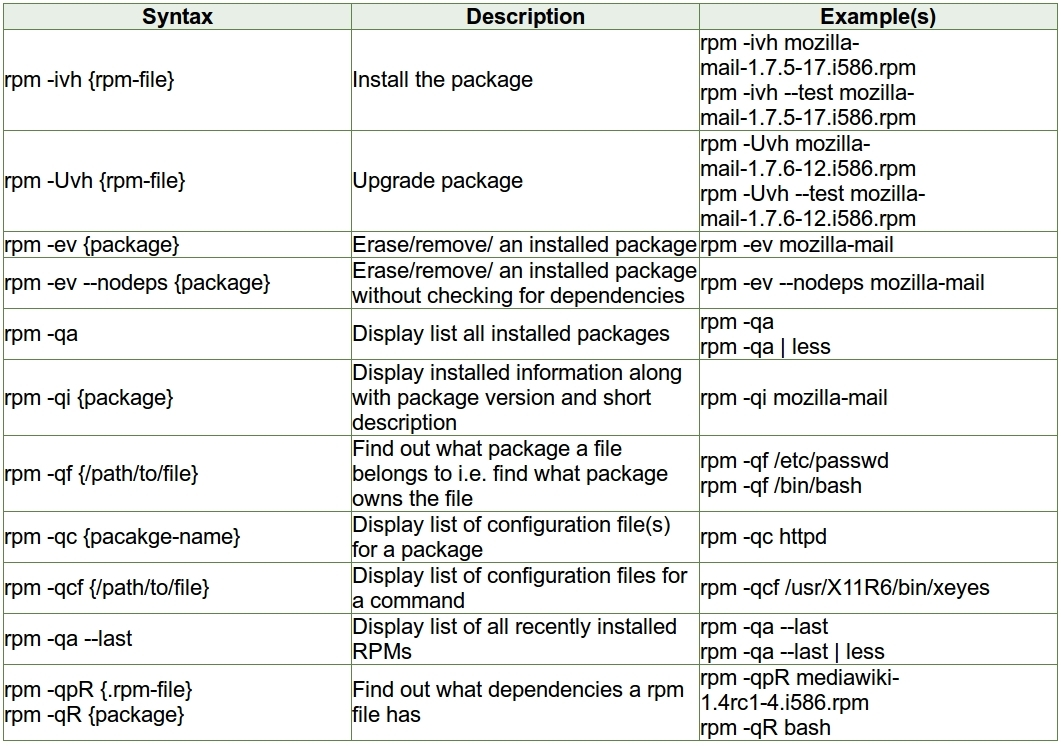
\includegraphics[width=8.8cm,height=7.5cm]{c6_rpm_01.png}}
	      \item RPM:rpm软件包管理器
	      \item Yum:RPM的前端
	    \end{itemize}
	  \item \textcolor{red}{\textbf{【难点】}}RPM\textcolor{red}{(实例讲解、操作演示)}
	    \begin{itemize}
	    \vspace*{-10pt}
		\begin{multicols}{2}
	      \item 功能
		\begin{itemize}
		  \item 查询:-q
		  \item 校验:-V
		  \item 安装:-i
		  \item 删除:-e
		  \item 升级:-U
		\end{itemize}
	      \item 选项
		\begin{itemize}
		  \item 通用:-v
		  \item 选择:-a,-f,-p
		  \item 查询:-l,-i,-c,-d,-R,-s
		  \item 安装:-h,-\ -nodeps,-\ -prefix,-\ -test,-\ -replacepkgs,-\ -force
		\end{itemize}
	      \end{multicols}
	    \vspace*{-10pt}
	    \end{itemize}
	  \item \textcolor{red}{\textbf{【重点】}}Yum\textcolor{red}{(实例讲解、操作演示)}
	    \vspace*{-10pt}
	    \begin{figure}[h]
	      \centering
	      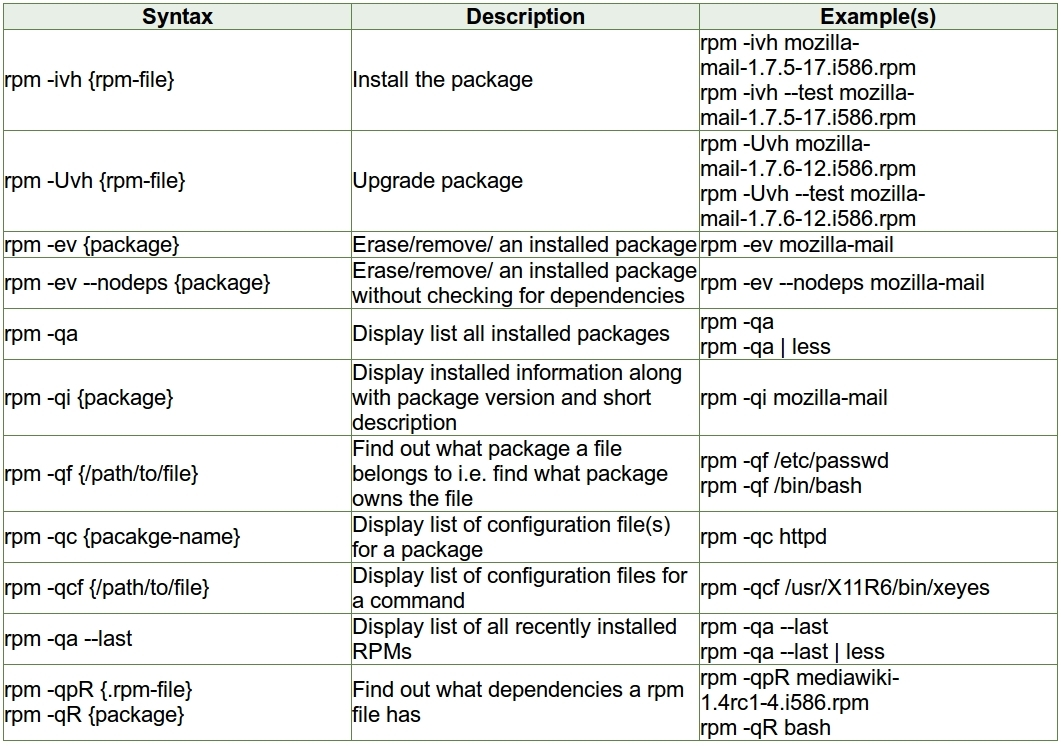
\includegraphics[width=10.5cm,height=6cm]{c6_rpm_01.png}
	      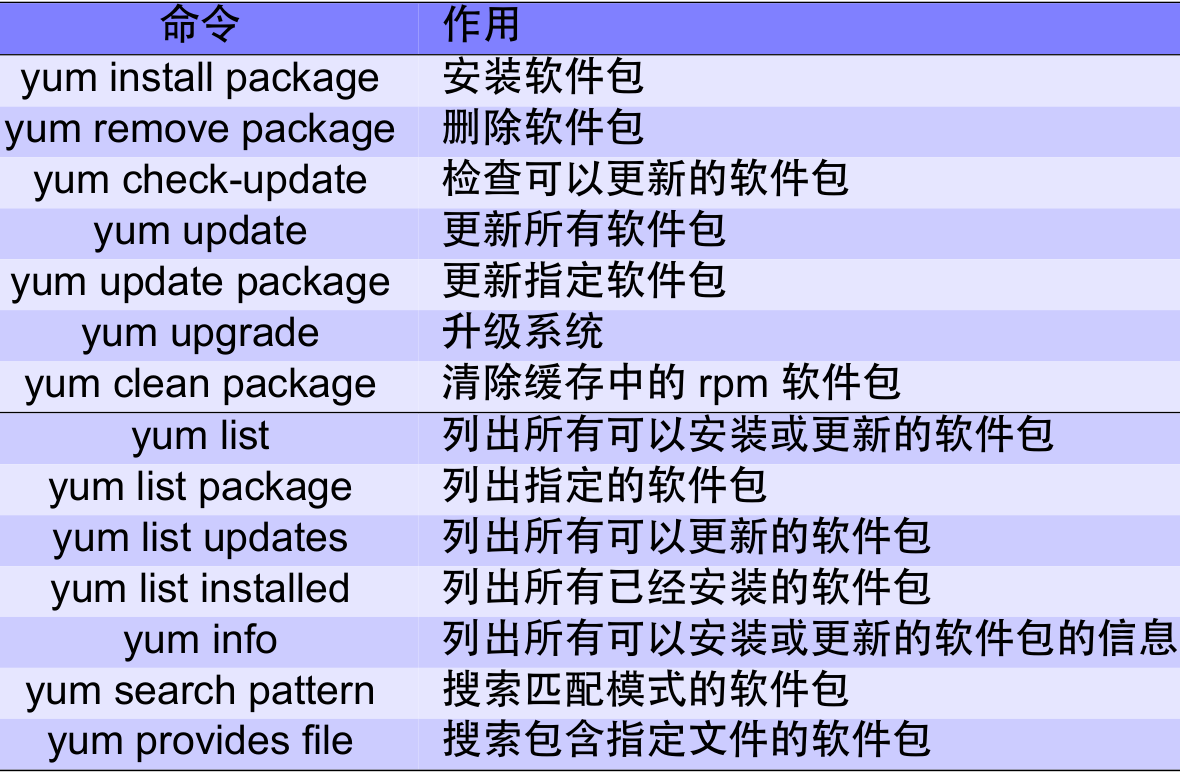
\includegraphics[width=7cm,height=6cm]{c6_yum.png}
	    \end{figure}
	    \vspace*{-10pt}
	\end{enumerate}
      \item 比较
    \end{enumerate}

  \item 源代码安装(40分钟)
    \begin{enumerate}
      \item 源代码
	\begin{itemize}
	  \item 源代码:创建软件的原始数据,源代码+文档
	  \item 开放源代码:以源代码形式提供的软件,带有特定许可条款
	\end{itemize}


\otherTail
\newpage
\otherHeader


	    \vspace*{-10pt}
	    \begin{figure}[h]
	      \centering
	      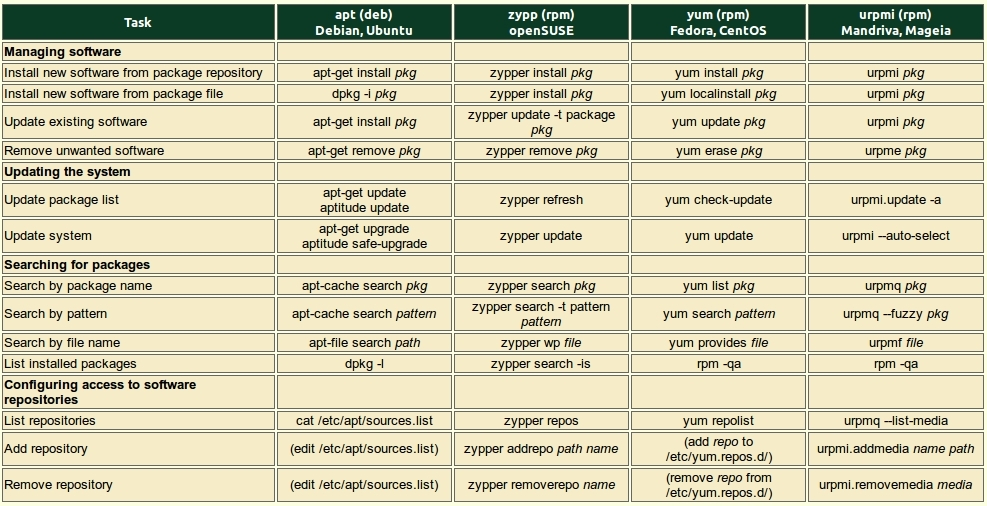
\includegraphics[width=17cm]{c6_compare_all_01.png}
	    \end{figure}
	    \vspace*{-10pt}

      \item 开源许可证
	\begin{itemize}
\parpic[fr]{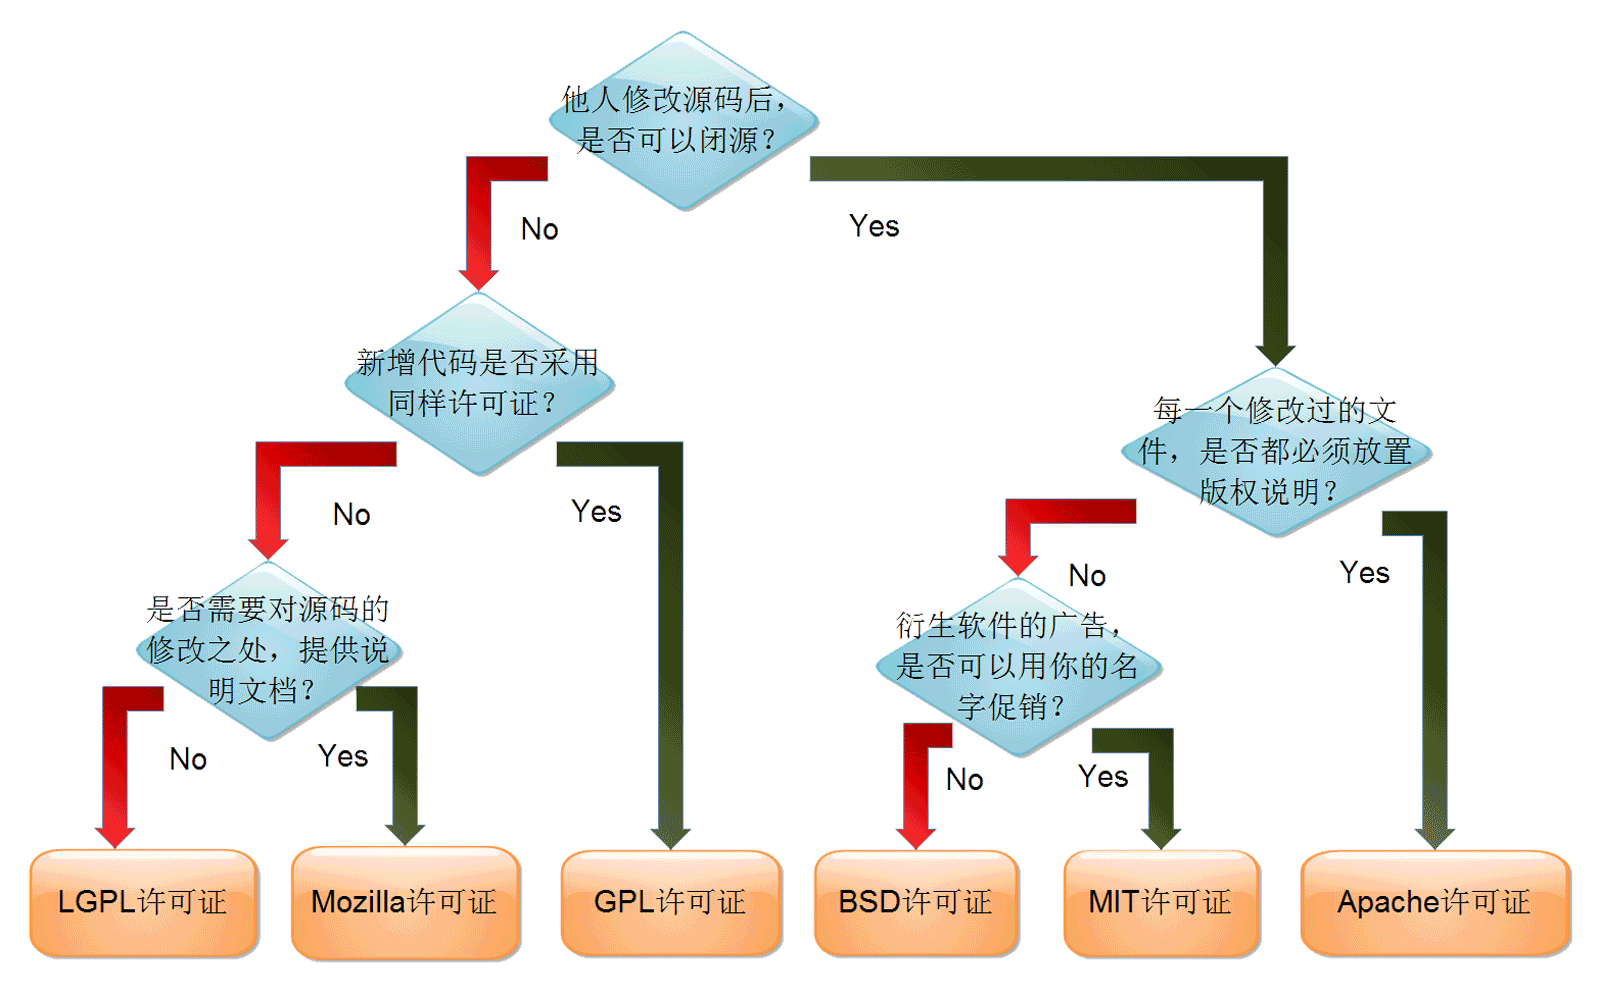
\includegraphics[width=8.5cm]{c6_license_choose_01.png}}
	  \item BSD许可证:copycenter
	  \item GPL许可证:copyleft
	    \begin{itemize}
              \item 使用的自由:使用不受任何限制
	      \item 研究的自由:获得源代码并研究
	      \item 散布的自由:复制散布软件
	      \item 改良的自由:改良软件并散布
	    \end{itemize}
	\end{itemize}
      \item 选择软件:LATEST,alpha,beta,……
      \item 下载软件:浏览器,FTP客户端,命令行
      \item \textcolor{red}{\textbf{【重点】}}安装软件\textcolor{red}{(实例讲解、操作演示)}
	\begin{itemize}
	  \item 准备工作
	    \begin{enumerate}
              \item 下载软件:\verb|wget -c software.tar.gz|
	      \item 提取文件:\verb|tar -xzvf software.tar.gz|
	      \item 切换目录:\verb|cd software|
	    \end{enumerate}
	  \item 安装软件
	    \begin{enumerate}
              \item 配置环境:\verb|./configure|
	      \item 编译软件:\verb|make|
	      \item 安装软件:\verb|make install|
	    \end{enumerate}
	  \item 其他工作
	    \begin{itemize}
	      \item 阅读软件的指南或说明:\verb|vim INSTALL|,或\verb|vim README|
	      \item 指定软件的安装目录:\verb|./configure --prefix=PATH|
	      \item 安装软件前进行测试:\verb|make test|,或\verb|make check|
	      \item 以超级用户身份安装软件:\verb|sudo make install|
	      \item 删除编译产生的临时文件:\verb|make clean|
	    \end{itemize}
	\end{itemize}
    \end{enumerate}

  \item 脚本安装(5分钟)
    \vspace*{-10pt}
    \begin{multicols}{2}
    \begin{enumerate}
      \item 下载软件:\verb|wget -c X.tar.gz|
      \item 提取文件:\verb|tar -xzvf X.tar.gz|
      \item 切换目录:\verb|cd software|
      \item 查阅说明:\verb|vim README|
      \item 安装软件:\verb|./setup.sh|,或\verb|./install.sh|
    \end{enumerate}
    \end{multicols}
    \vspace*{-10pt}


\otherTail
\newpage
\otherHeader


  \item 总结与答疑(5分钟)
    \begin{enumerate}
      \item 知识点
	\begin{itemize}
          \item 软件包管理:软件包的类型,管理系统
          \item 二进制软件包管理:dpkg与APT,RPM与Yum
          \item 源代码安装:开源许可证,版本选择,安装步骤
          \item 脚本安装:基本步骤
	\end{itemize}
      \item 技能
	\begin{itemize}
          \item Ubuntu中的软件管理
          \item CentOS中的软件管理
          \item 通过源代码安装软件
	\end{itemize}
    \end{enumerate}

\end{enumerate}

\otherTail


\end{document}

